\documentclass[12pt]{aber-thesis}

%load any additional packages
\usepackage{amsfonts,amsmath,amssymb,amstext}

\usepackage[hang]{subfigure}
\usepackage{float}
\usepackage{multirow}

\usepackage{graphicx}
\usepackage{epstopdf}

\usepackage{xcolor}
\usepackage{fixltx2e}
\usepackage{booktabs}

\usepackage[font=footnotesize,margin=1cm]{caption}
\captionsetup{labelfont=bf}
\captionsetup[table]{singlelinecheck=false}
\graphicspath{{figs/}}

%\usepackage[sort,authoryear]{natbib}
\usepackage[sort,numbers]{natbib}

\usepackage{setspace}
\usepackage{microtype}
\usepackage[all]{nowidow}

\usepackage[linktocpage]{hyperref}

\setkeys{Gin}{width=0.66\linewidth}

\title{My Title \\[1ex]     %your thesis title,
        title title}   %note \\[1ex] is a line break in the title

\author{Author Name}             %your name
\college{The Department of Physics}  %your college

%\renewcommand{\submittedtext}{change the default text here if needed}
\degreename{Doctor of Philosophy}     %the degree
\degreedate{March 2015}         %the degree date

%end the preamble and start the document
\begin{document}

%this baselineskip gives sufficient line spacing for an examiner to easily
%markup the thesis with comments
\baselineskip=24pt plus1pt

%set the number of sectioning levels that get number and appear in the contents
\setcounter{secnumdepth}{2}
\setcounter{tocdepth}{2}

\maketitle                  % create a title page from the preamble info
\begin{originality}

Word Count of thesis: 26,448 Words

\textbf{Declaration}

{\setstretch{1.0}
This work has not previously been accepted in substance for any degree and is not being concurrently submitted in candidature for any degree. \par }

Signed ...................................................................... (candidate)

Date ........................................................................

\textbf{Statement 1}

{\setstretch{1.0}
This thesis is the result of my own investigations, except where otherwise stated. Where correction services have been used, the extent and nature of the correction is clearly marked in a footnote(s). \par }

{\setstretch{1.0}
Other sources are acknowledged by footnotes giving explicit references. \\*
A bibliography is appended. \par }

Signed ..................................................................... (candidate)

Date ........................................................................

\textbf{Statement 2}

{\setstretch{1.0}
I hereby give consent for my thesis, if accepted, to be available for photocopying and for inter-library loan, and for the title and summary to be made available to outside organisations. \par }

Signed ..................................................................... (candidate)

Date ........................................................................

\end{originality}       % include a statement of originality
\begin{dedication}
This thesis is dedicated to someone special,\\
for a special reason.\\
\end{dedication}        % include a dedication.tex file
\begin{acknowledgements}
plenty of waffle, plenty of waffle, plenty of waffle, plenty of waffle,
plenty of waffle, plenty of waffle, plenty of waffle, plenty of waffle.
\end{acknowledgements}   % include an acknowledgements.tex file
\begin{abstract}
plenty of waffle, plenty of waffle, plenty of waffle, plenty of waffle,
plenty of waffle, plenty of waffle, plenty of waffle, plenty of waffle.
plenty of waffle, plenty of waffle, plenty of waffle, plenty of waffle.
\end{abstract}          % include the abstract

\begin{romanpages}          % start roman page numbering
\tableofcontents            % generate and include a table of contents
\listoffigures              % generate and include a list of figures
\listoftables               % generate and include a list of tables	
\end{romanpages}            % end roman page numbering

%now include the files of latex for each of the chapters etc
\chapter{Some Title}
\textbf{\bibentry{example-ref2015}}

\section{Some other title}
\subsection{more titles}
\subsubsection{titles}

Lorem ipsum dolor sit amet, consectetur adipiscing elit, sed do eiusmod tempor incididunt ut labore et dolore magna aliqua. Ut enim ad minim veniam, quis nostrud exercitation ullamco laboris nisi ut aliquip ex ea commodo consequat. Duis aute irure dolor in reprehenderit in voluptate velit esse cillum dolore eu fugiat nulla pariatur. Excepteur sint occaecat cupidatat non proident, sunt in culpa qui officia deserunt mollit anim id est laborum.
\chapter{Some Title}

\section{Some other title}
\subsection{more titles}
\subsubsection{titles}

Lorem ipsum dolor sit amet, consectetur adipiscing elit, sed do eiusmod tempor incididunt ut labore et dolore magna aliqua. Ut enim ad minim veniam, quis nostrud exercitation ullamco laboris nisi ut aliquip ex ea commodo consequat. Duis aute irure dolor in reprehenderit in voluptate velit esse cillum dolore eu fugiat nulla pariatur. Excepteur sint occaecat cupidatat non proident, sunt in culpa qui officia deserunt mollit anim id est laborum.
\chapter{Some Title}

\section{Some other title}
\subsection{more titles}
\subsubsection{ so many titles}

Lorem ipsum dolor sit amet, consectetur adipiscing elit, sed do eiusmod tempor incididunt ut labore et dolore magna aliqua. Ut enim ad minim veniam, quis nostrud exercitation ullamco laboris nisi ut aliquip ex ea commodo consequat. Duis aute irure dolor in reprehenderit in voluptate velit esse cillum dolore eu fugiat nulla pariatur. Excepteur sint occaecat cupidatat non proident, sunt in culpa qui officia deserunt mollit anim id est laborum.
\chapter{Some Title}

\section{Some other title}
\subsection{more titles}
\subsubsection{titles}

Lorem ipsum dolor sit amet, consectetur adipiscing elit, sed do eiusmod tempor incididunt ut labore et dolore magna aliqua. Ut enim ad minim veniam, quis nostrud exercitation ullamco laboris nisi ut aliquip ex ea commodo consequat. Duis aute irure dolor in reprehenderit in voluptate velit esse cillum dolore eu fugiat nulla pariatur. Excepteur sint occaecat cupidatat non proident, sunt in culpa qui officia deserunt mollit anim id est laborum.
\chapter{Some Title}

\section{Some other title}
\subsection{more titles}
\subsubsection{so many titles}

Lorem ipsum dolor sit amet, consectetur adipiscing elit, sed do eiusmod tempor incididunt ut labore et dolore magna aliqua. Ut enim ad minim veniam, quis nostrud exercitation ullamco laboris nisi ut aliquip ex ea commodo consequat. Lorem ipsum dolor sit amet, consectetur adipiscing elit, sed do eiusmod tempor incididunt ut labore et dolore magna aliqua. Ut enim ad minim veniam, quis nostrud exercitation ullamco laboris nisi ut aliquip ex ea commodo consequat. Lorem ipsum dolor sit amet, consectetur adipiscing elit, sed do eiusmod tempor incididunt ut labore et dolore magna aliqua. Ut enim ad minim veniam, quis nostrud exercitation ullamco laboris nisi ut aliquip ex ea commodo consequat. Lorem ipsum dolor sit amet, consectetur adipiscing elit, sed do eiusmod tempor incididunt ut labore et dolore magna aliqua. Ut enim ad minim veniam, quis nostrud exercitation ullamco laboris nisi ut aliquip ex ea commodo consequat.
\begin{figure}[t]
	\centering
	\hfill
	{\subfigcapskip = 6pt \subfigure [Example 1] {
			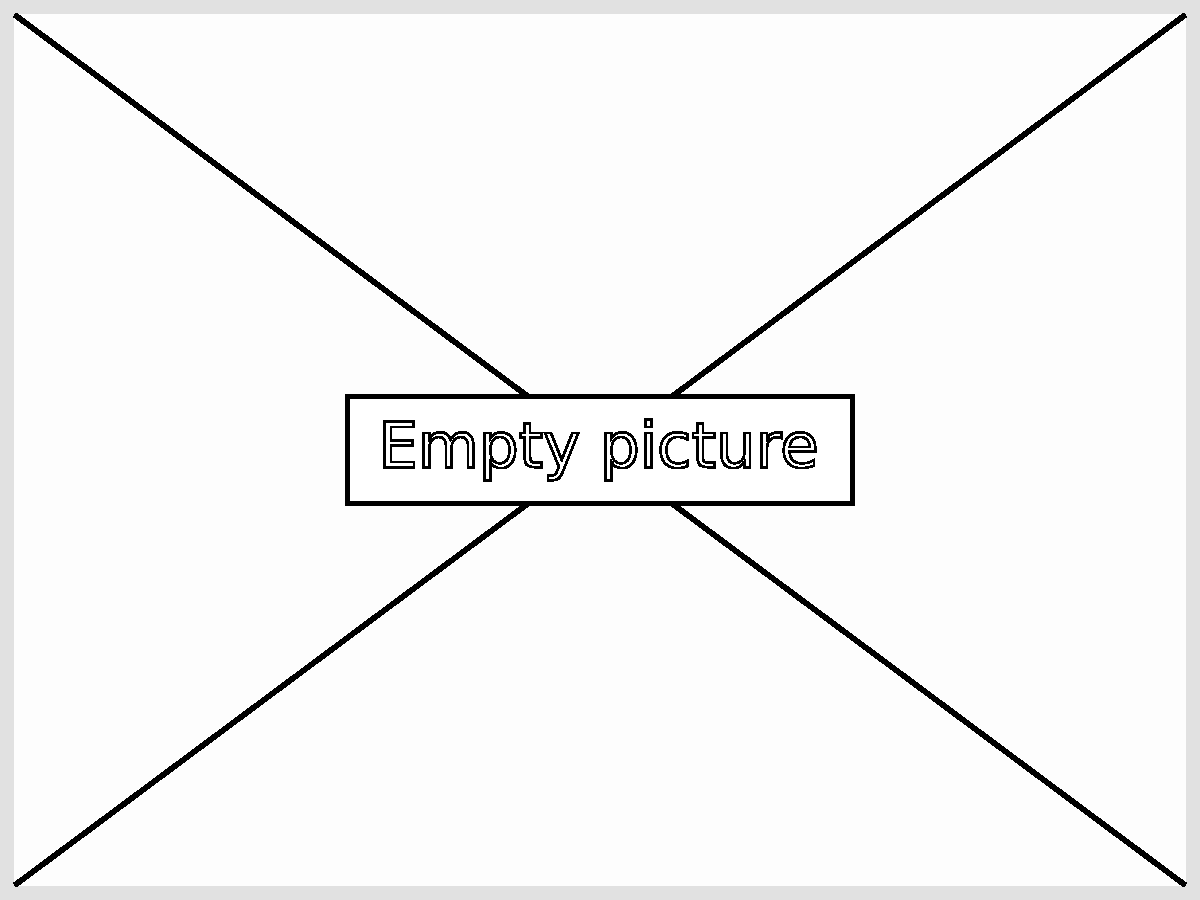
\includegraphics[width=0.47\linewidth]{figs/empty.pdf}
			\label{fig:empty1}
	}}
	\hfill
	{\subfigcapskip = 6pt \subfigure [Example 2] {
			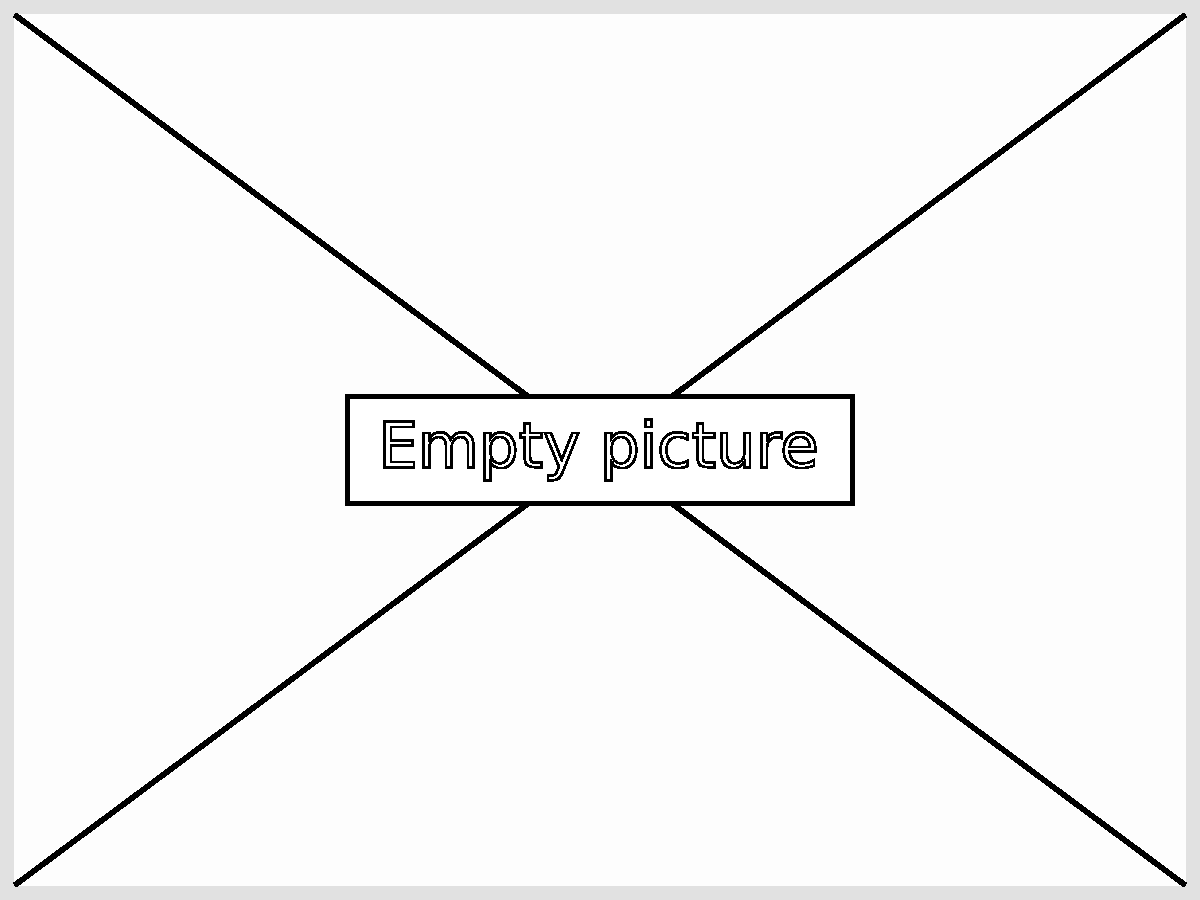
\includegraphics[width=0.47\linewidth]{figs/empty.pdf}
			\label{fig:empty2}
	}}
	\hfill
	\vspace{6pt}
	\caption{Example of including two pictures.}
	\label{fig:empty3}
\end{figure}
Lorem ipsum dolor sit amet, consectetur adipiscing elit, sed do eiusmod tempor incididunt ut labore et dolore magna aliqua. Ut enim ad minim veniam, quis nostrud exercitation ullamco laboris nisi ut aliquip ex ea commodo consequat. Lorem ipsum dolor sit amet, consectetur adipiscing elit, sed do eiusmod tempor incididunt ut labore et dolore magna aliqua. Ut enim ad minim veniam, quis nostrud exercitation ullamco laboris nisi ut aliquip ex ea commodo consequat. Lorem ipsum dolor sit amet, consectetur adipiscing elit, sed do eiusmod tempor incididunt ut labore et dolore magna aliqua. Ut enim ad minim veniam, quis nostrud exercitation ullamco laboris nisi ut aliquip ex ea commodo consequat. Lorem ipsum dolor sit amet, consectetur adipiscing elit, sed do eiusmod tempor incididunt ut labore et dolore magna aliqua. Ut enim ad minim veniam, quis nostrud exercitation ullamco laboris nisi ut aliquip ex ea commodo consequat. Lorem ipsum dolor sit amet, consectetur adipiscing elit, sed do eiusmod tempor incididunt ut labore et dolore magna aliqua. Ut enim ad minim veniam, quis nostrud exercitation ullamco laboris nisi ut aliquip ex ea commodo consequat.

Duis aute irure dolor in reprehenderit in voluptate velit esse cillum dolore eu fugiat nulla pariatur. Excepteur sint occaecat cupidatat non proident, sunt in culpa qui officia deserunt mollit anim id est laborum in Fig~\ref{fig:empty4}. Lorem ipsum dolor sit amet, consectetur adipiscing elit, sed do eiusmod tempor incididunt ut labore et dolore magna aliqua. Ut enim ad minim veniam, quis nostrud exercitation ullamco laboris nisi ut aliquip ex ea commodo consequat. Lorem ipsum dolor sit amet, consectetur adipiscing elit, sed do eiusmod tempor incididunt ut labore et dolore magna aliqua. Ut enim ad minim veniam, quis nostrud exercitation ullamco laboris nisi ut aliquip ex ea commodo consequat.
\begin{figure}[t]
	\centering
	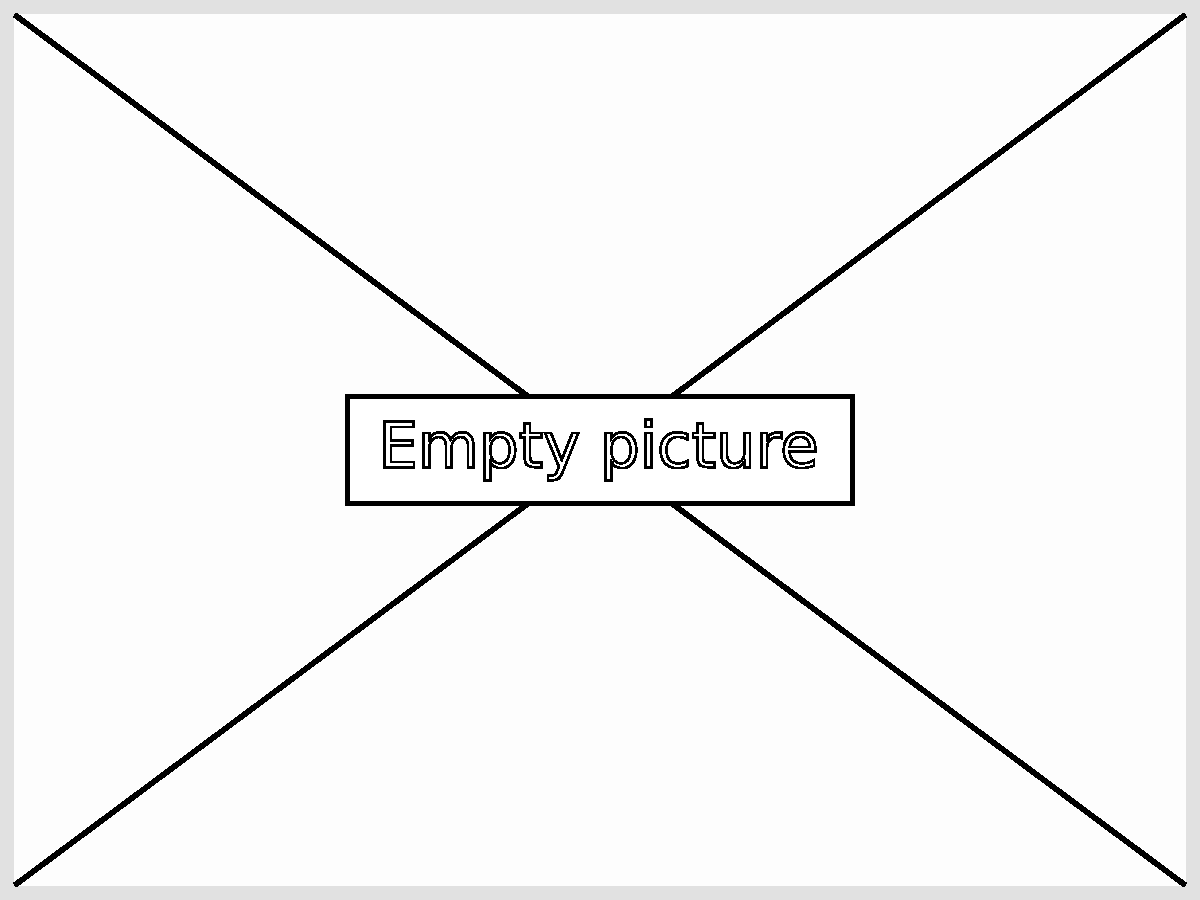
\includegraphics[width=0.80\linewidth]{figs/empty.pdf}
	\vspace{6pt}
	\caption{Example of including just one picture.}
	\label{fig:empty4}
\end{figure}
Lorem ipsum dolor sit amet, consectetur adipiscing elit, sed do eiusmod tempor incididunt ut labore et dolore magna aliqua. Ut enim ad minim veniam, quis nostrud exercitation ullamco laboris nisi ut aliquip ex ea commodo consequat. Lorem ipsum dolor sit amet, consectetur adipiscing elit, sed do eiusmod tempor incididunt ut labore et dolore magna aliqua. Ut enim ad minim veniam, quis nostrud exercitation ullamco laboris nisi ut aliquip ex ea commodo consequat. Lorem ipsum dolor sit amet, consectetur adipiscing elit, sed do eiusmod tempor incididunt ut labore et dolore magna aliqua. Ut enim ad minim veniam, quis nostrud exercitation ullamco laboris nisi ut aliquip ex ea commodo consequat.
\begin{table}[t]
	\renewcommand{\arraystretch}{1.5}
	\centering
	\begin{tabular}{c|c}
	\textbf{Header1} &  \textbf{Header2} \\
	\hline\hline
	Cell 1 & Cell 2 \\	
	\hline
	Cell 3 & Cell 4 \\	
	\end{tabular}
	\vspace{6pt}
	\caption{Example of table.}
	\label{tab:empty1}
\end{table}

Lorem ipsum dolor sit amet, consectetur adipiscing elit, sed do eiusmod tempor incididunt ut labore et dolore magna aliqua. Ut enim ad minim veniam, quis nostrud exercitation ullamco laboris nisi ut aliquip ex ea commodo consequat. Lorem ipsum dolor sit amet, consectetur adipiscing elit, sed do eiusmod tempor incididunt ut labore et dolore magna aliqua. Ut enim ad minim veniam, quis nostrud exercitation ullamco laboris nisi ut aliquip ex ea commodo consequat. Lorem ipsum dolor sit amet, consectetur adipiscing elit, sed do eiusmod tempor incididunt ut labore et dolore magna aliqua. Ut enim ad minim veniam, quis nostrud exercitation ullamco laboris nisi ut aliquip ex ea commodo consequat.
\begin{figure}[p]
	\centering
	{\subfigcapskip = 6pt \subfigure [Example 5] {
			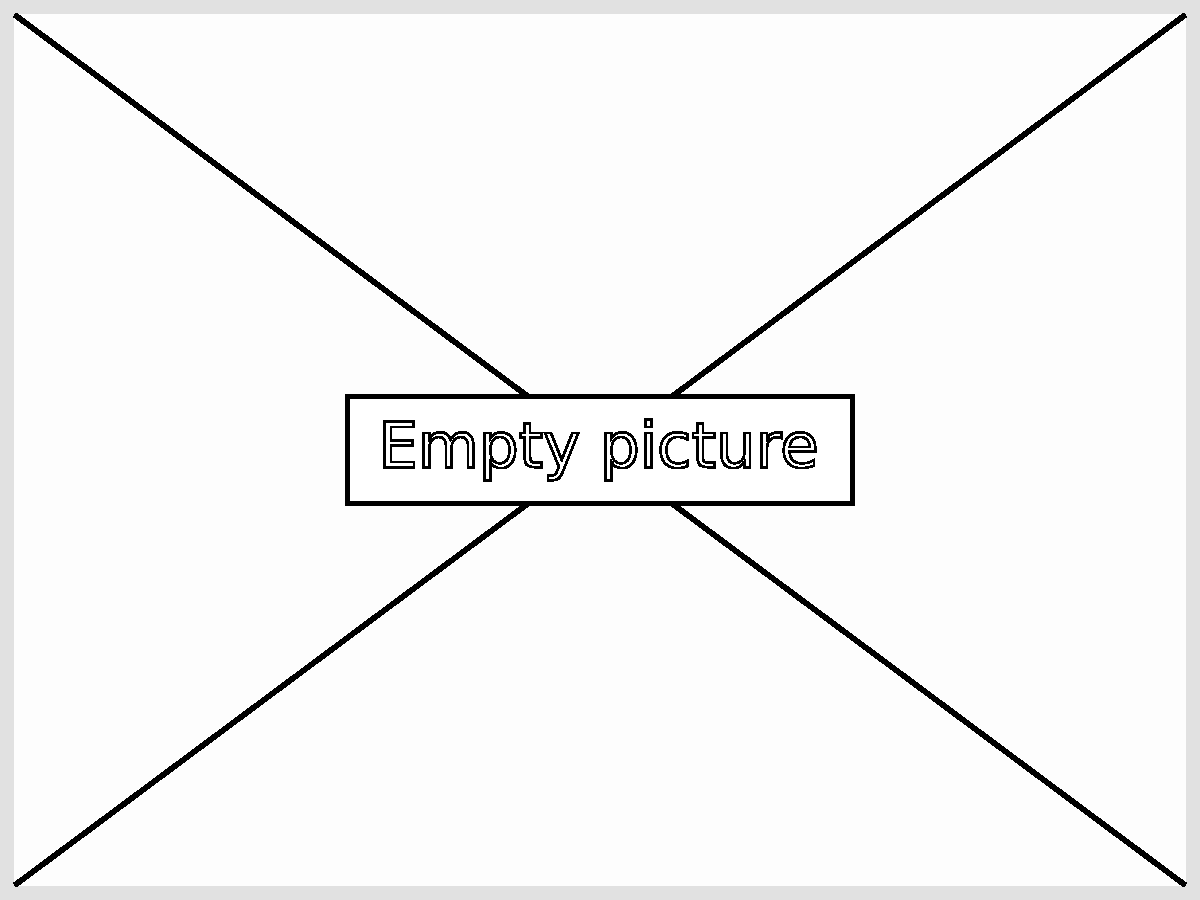
\includegraphics[height=8.5cm]{figs/empty.pdf}
			\label{fig:empty5}
	}}
	\\ \vspace{2cm}
	{\subfigcapskip = 6pt \subfigure [Example 6] {
			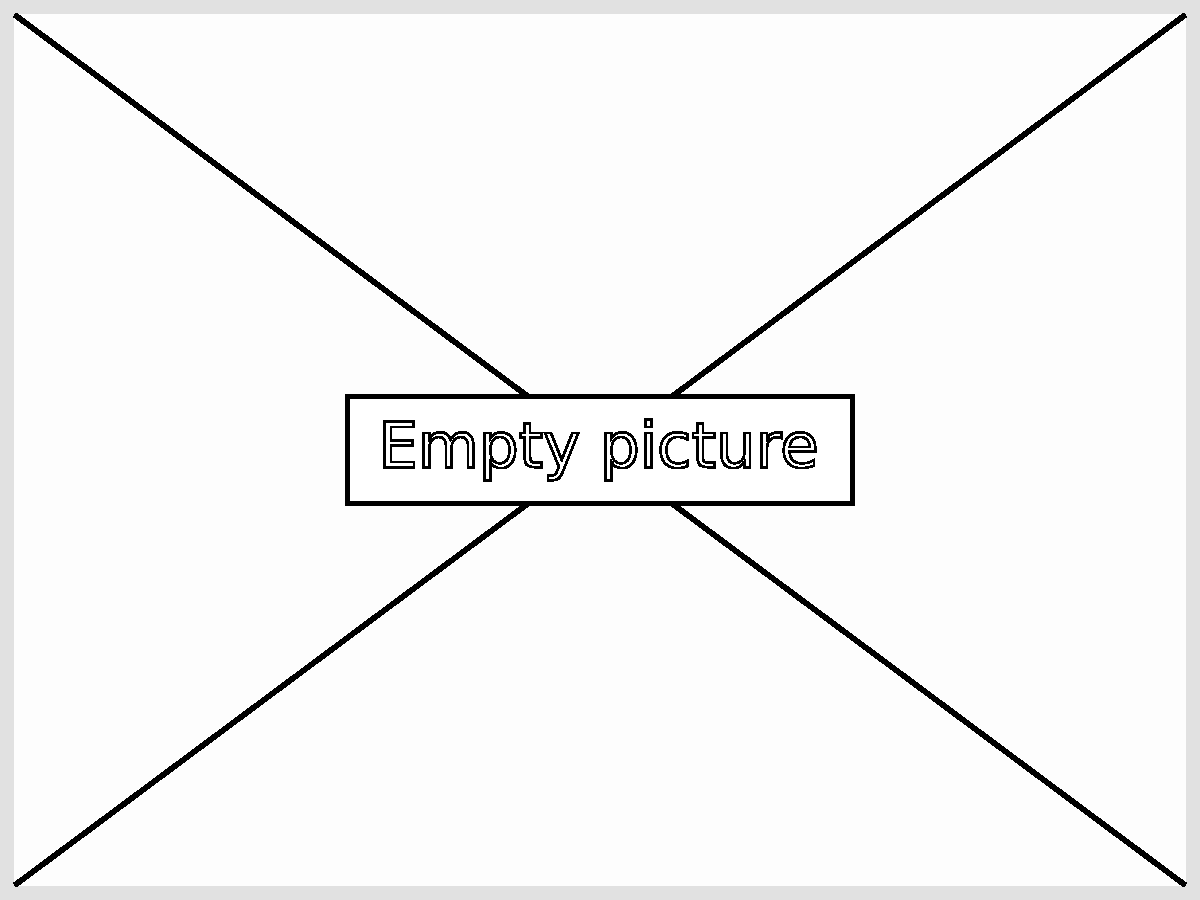
\includegraphics[height=8.5cm]{figs/empty.pdf}
			\label{fig:empty6}
	}}
	\vspace{6pt}
	\caption{Example of a page with two pictures.}
	\label{fig:empty7}
\end{figure}
Lorem ipsum dolor sit amet, consectetur adipiscing elit, sed do eiusmod tempor incididunt ut labore et dolore magna aliqua. Ut enim ad minim veniam, quis nostrud exercitation ullamco laboris nisi ut aliquip ex ea commodo consequat. Lorem ipsum dolor sit amet, consectetur adipiscing elit, sed do eiusmod tempor incididunt ut labore et dolore magna aliqua. Ut enim ad minim veniam, quis nostrud exercitation ullamco laboris nisi ut aliquip ex ea commodo consequat. Lorem ipsum dolor sit amet, consectetur adipiscing elit, sed do eiusmod tempor incididunt ut labore et dolore magna aliqua. Ut enim ad minim veniam, quis nostrud exercitation ullamco laboris nisi ut aliquip ex ea commodo consequat.
\chapter{Conclusions}

Lorem ipsum dolor sit amet, consectetur adipiscing elit, sed do eiusmod tempor incididunt ut labore et dolore magna aliqua. Ut enim ad minim veniam, quis nostrud exercitation ullamco laboris nisi ut aliquip ex ea commodo consequat. Duis aute irure dolor in reprehenderit in voluptate velit esse cillum dolore eu fugiat nulla pariatur. Excepteur sint occaecat cupidatat non proident, sunt in culpa qui officia deserunt mollit anim id est laborum.

%now enable appendix numbering format and include any appendices
\appendix
\chapter{Appendix I}

Lorem ipsum dolor sit amet, consectetur adipiscing elit, sed do eiusmod tempor incididunt ut labore et dolore magna aliqua. Ut enim ad minim veniam, quis nostrud exercitation ullamco laboris nisi ut aliquip ex ea commodo consequat. Duis aute irure dolor in reprehenderit in voluptate velit esse cillum dolore eu fugiat nulla pariatur. Excepteur sint occaecat cupidatat non proident, sunt in culpa qui officia deserunt mollit anim id est laborum.
\chapter{Appendix II}

Lorem ipsum dolor sit amet, consectetur adipiscing elit, sed do eiusmod tempor incididunt ut labore et dolore magna aliqua. Ut enim ad minim veniam, quis nostrud exercitation ullamco laboris nisi ut aliquip ex ea commodo consequat. Duis aute irure dolor in reprehenderit in voluptate velit esse cillum dolore eu fugiat nulla pariatur. Excepteur sint occaecat cupidatat non proident, sunt in culpa qui officia deserunt mollit anim id est laborum.

%next line adds the Bibliography to the contents page
\addcontentsline{toc}{chapter}{Bibliography}

\bibliography{references}
\bibliographystyle{agsm-mod}

\end{document}
